
\vspace{-0.3cm}
\begin{IEEEbiography}[{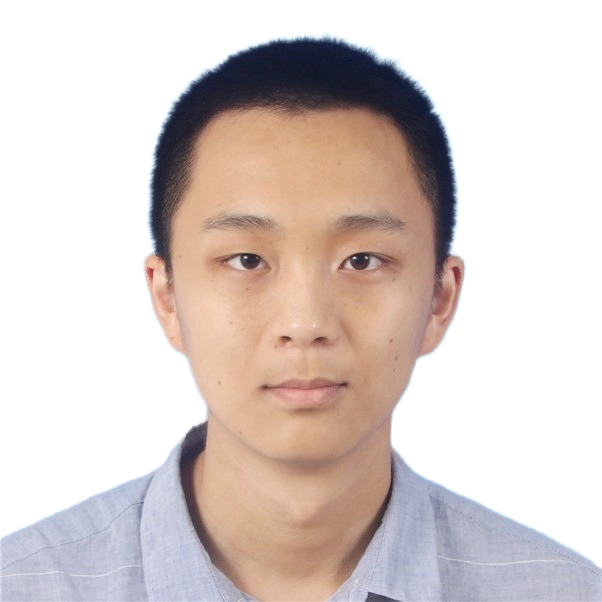
\includegraphics[width=1in,height=1.25in,clip,keepaspectratio]{photos/yuncong.png}}]{Yuncong Hong}
    received the B.Eng. degree in Electrical and Electronic Engineering from the Southern University of Science and Technology (SUSTech), China, in 2018, and the Ph.D. degree in Computer Science from The University of Hong Kong (HKU) in 2024. His research interests lie in WLAN system optimization, edge computing, and distributed networks, with a focus on improving network performance and scalability in real-world applications.
\end{IEEEbiography}
\vspace{-1cm}

\begin{IEEEbiography}[{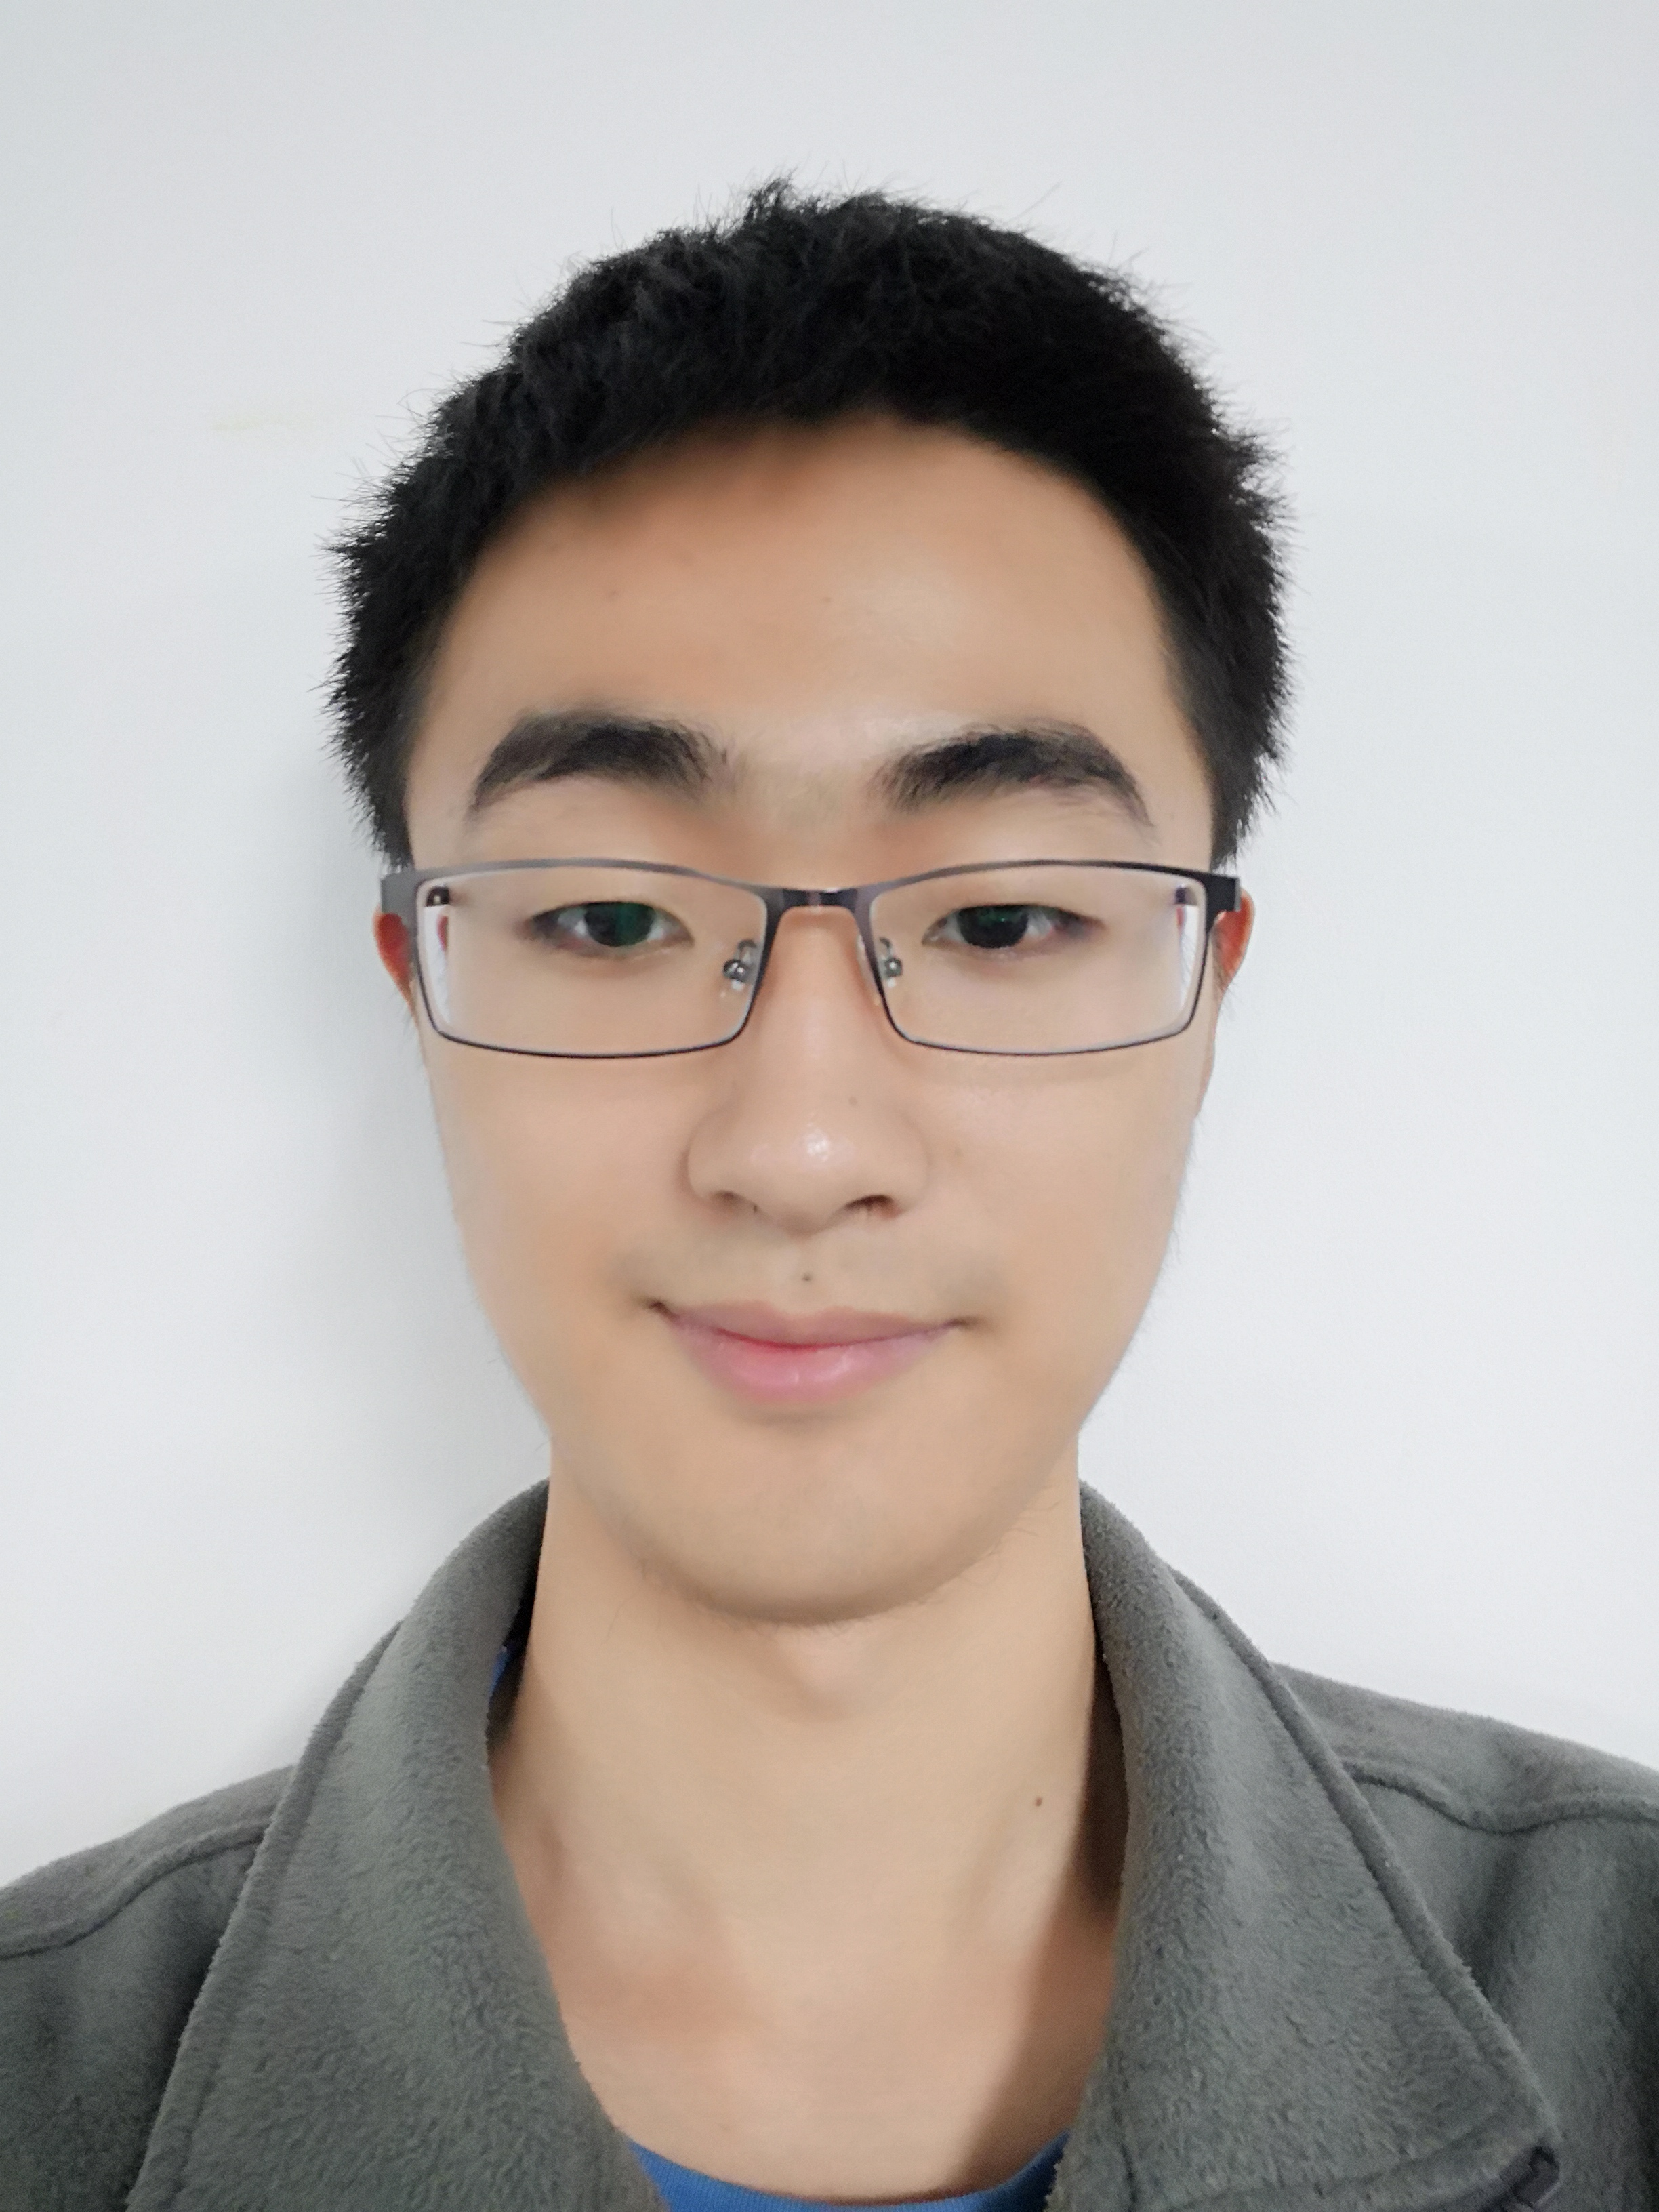
\includegraphics[width=1in,height=1.25in,clip,keepaspectratio]{photos/lv.jpg}}]{Bojie Lv}
    received the B.E. degree in communication engineering from the Southern University of Science and Technology (SUSTech), Shenzhen, China, in 2018, and the M.Phil. degree (Hons.) in information and communication engineering from Harbin Institute of Technology, Harbin, China, in 2020. He is currently pursuing the Ph.D. degree in mathematics with SUSTech. His research interests include stochastic optimization and resource allocation in the wireless networks.
\end{IEEEbiography}
\vspace{-1cm}

\begin{IEEEbiography}
[{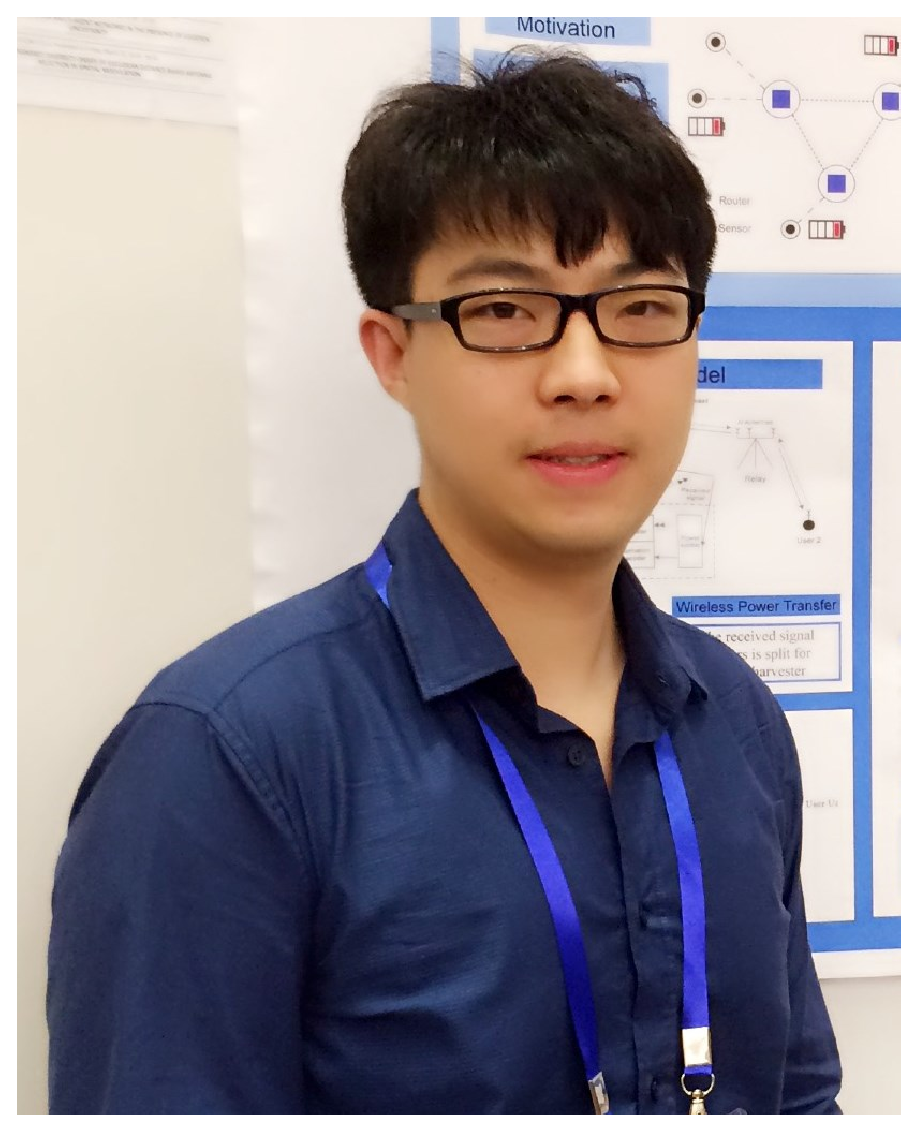
\includegraphics[width=1in, height=1.25in, clip, keepaspectratio]{photos/shuaiwang.eps}}]{Shuai Wang} (M'19--SM’24)
received the Ph.D. degree in Electrical and Electronic Engineering from The University of Hong Kong (HKU) in 2018. He is now an Associate Professor with the Shenzhen Institutes of Advanced Technology (SIAT), Chinese Academy of Sciences, where he leads the Intelligent Networked Vehicle Systems (INVS) Laboratory. His research interests lie at the intersection of autonomous systems and wireless communications. He has published more than 100 journal and conference papers. He has received best paper awards from IEEE ICC, SPCC, and ICDCSW.
\end{IEEEbiography}
\vspace{-1cm}

\begin{IEEEbiography}[{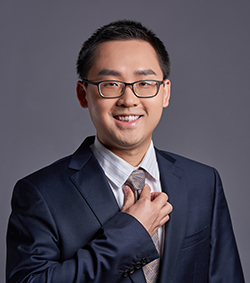
\includegraphics[width=1in,height=1.25in,clip,keepaspectratio]{photos/ruiwang.jpg}}]{Rui Wang}
    (Member, IEEE) received the B.S. degree from the University of Science and Technology of China in 2004, and the Ph.D. degree in wireless communications from The Hong Kong University of Science and Technology in 2008.
	From 2009 to 2012, he was a Senior Research Engineer with Huawei Technologies, Co., Ltd.
	Since 2012, he has joined the Southern University of Science and Technology of China as an Associate Professor.
	He has research experience in both academia and industry.
	He has authored over 100 papers in top-level IEEE journals and flagship international conferences, especially in the area of wireless radio resource optimization and interference management.
	He has contributed over 20 U.S. patent applications and over 100 Chinese patent applications (50 of them have been granted).
\end{IEEEbiography}
\vspace{-1cm}

\begin{IEEEbiography}[{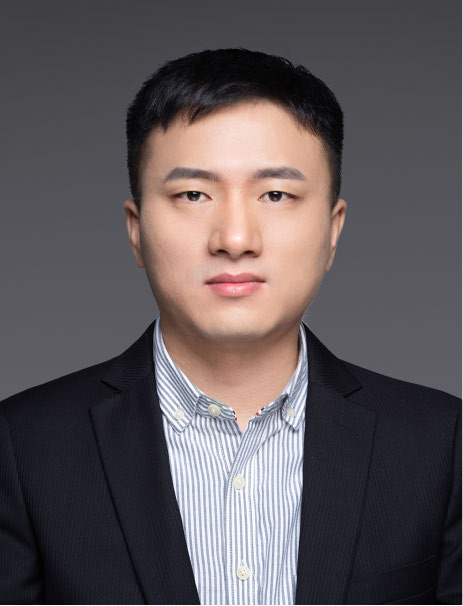
\includegraphics[width=1in,height=1.25in,clip,keepaspectratio]{photos/haisheng.jpg}}]{Haisheng Tan}
    (Senior Member, IEEE) received the B.E. degree (Hons.) in software engineering and the B.S. degree (Hons.) in management from the University of Science and Technology of China (USTC), and the Ph.D. degree in computer science from The University of Hong Kong (HKU).
	He is currently a Professor with USTC.
	His research interests lie primarily in networking algorithm design and system implementation, where he has published over 100 papers in prestigious journals and conferences, including IEEE/ACM ToN, NSDI, INFOCOM, and EuroSys.
	He recently received the Best Paper Award in WASA'19, CWSN'20, PDCAT'20, and ICPADS'21.
\end{IEEEbiography}
\vspace{-1cm}

\begin{IEEEbiography}[{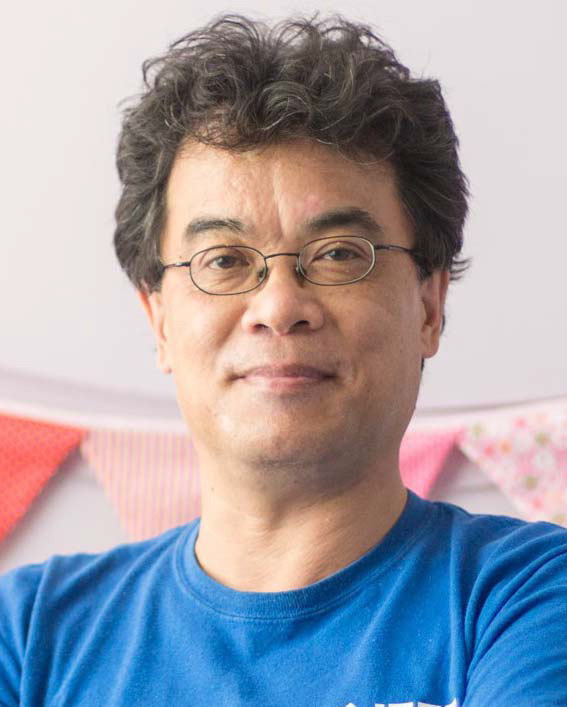
\includegraphics[width=1in,height=1.25in,clip,keepaspectratio]{photos/francis.png}}]{Francis~C.M.~Lau}
    received the Ph.D. degree from the Department of Computer Science, University of Waterloo.
	He was formerly Head of Department of Computer Science at The University of Hong Kong, China, where he now serves as an honorary professor.
	His research interests include computer systems, networks, AI, and application of computing in arts and music.
	He was the Editor-in-Chief of the Journal of Interconnection Networks from 2011 to 2020.
\end{IEEEbiography}
\vspace{-1cm}
